\documentclass{standalone}
\usepackage[most]{tcolorbox}
\usepackage{varwidth}
\usepackage{tikz}

\begin{document}
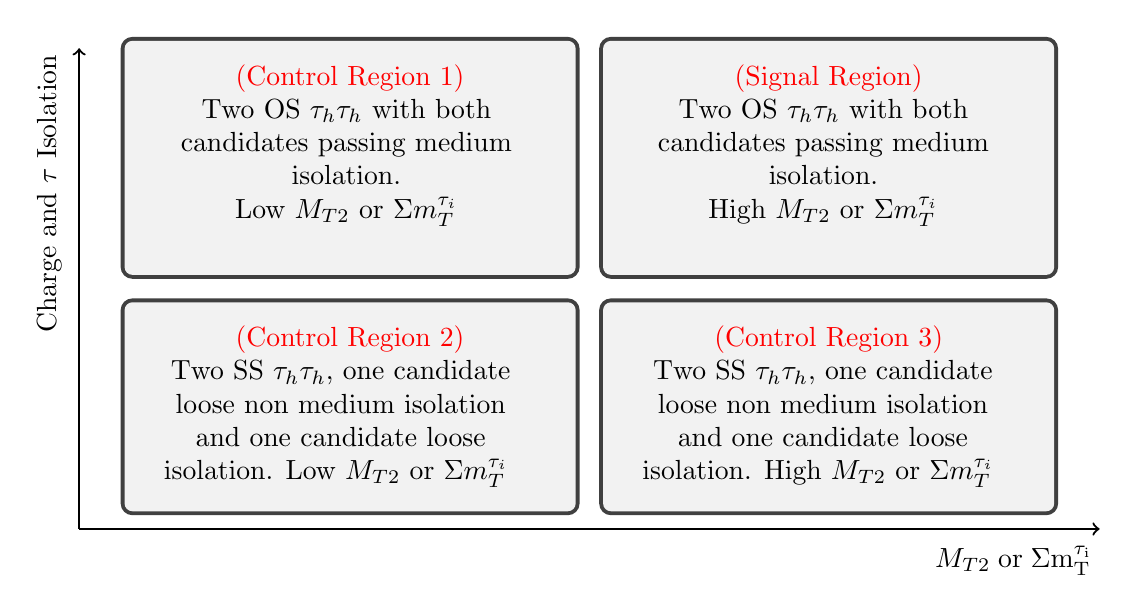
\begin{tikzpicture}[xscale=13.5,yscale=4.3]

  %axis -- coordinate (x axis mid)      coordinate (y axis mid) 
  \draw[thick,->] (0,0) -- (0.8,0) -- coordinate (x axis mid) (0.96,0);
  \draw[thick,->] (0,0) -- (0,0.56) -- coordinate (y axis mid) (0,1.42);

  \node[below=0.1cm] at (x axis mid) {$M_{T2}\;\rm{or}\;\Sigma m_T^{\tau_i}$};
  \node[rotate=90, above=0.1cm] at (y axis mid) {Charge and $\tau$ Isolation};

  \node [below right] at (.48,.71) {
    \begin{tcolorbox}[hbox]
      \begin{varwidth}{0.39\textwidth}
        \center{
          \color{red} (Control Region 3) \\
          \color{black} Two SS $\tau_{h}\tau_{h}$, one candidate loose non medium isolation\\
          and one candidate loose isolation. High $M_{T2}$ or $\Sigma m_T^{\tau_i}$
        }
      \end{varwidth}
    \end{tcolorbox}  
  };
  \node [above left] at (.48,.71) {
    \begin{tcolorbox}[hbox]
      \begin{varwidth}{0.39\textwidth}
        \center{
          \color{red} (Control Region 1) \\
          \color{black} Two OS $\tau_{h}\tau_{h}$ with both candidates passing medium isolation.\\
          Low $M_{T2}$ or $\Sigma m_T^{\tau_i}$\\
          \hspace{128bp}
        }
      \end{varwidth}
    \end{tcolorbox}
  };
  \node [below left] at (.48,.71) {
    \begin{tcolorbox}[hbox]
      \begin{varwidth}{0.39\textwidth}
        \center{
          \color{red} (Control Region 2) \\
          \color{black} Two SS $\tau_{h}\tau_{h}$, one candidate loose non medium isolation\\
          and one candidate loose isolation. Low $M_{T2}$ or $\Sigma m_T^{\tau_i}$
        }
      \end{varwidth}
    \end{tcolorbox}
  };
  \node [above right] at (.48,.71) {
    \begin{tcolorbox}[hbox]
      \begin{varwidth}{0.39\textwidth}
        \center{
          \color{red} (Signal Region) \\
          \color{black} Two OS $\tau_{h}\tau_{h}$ with both candidates passing medium isolation.\\
          High $M_{T2}$ or $\Sigma m_T^{\tau_i}$\\
          \hspace{127bp}
        }
      \end{varwidth}
    \end{tcolorbox}
  };
\end{tikzpicture}
\end{document}

